\documentclass[10pt]{article}
\usepackage[polish]{babel}
\usepackage[utf8]{inputenc}
\usepackage[T1]{fontenc}
\usepackage{graphicx}
\usepackage[export]{adjustbox}
\graphicspath{ {./images/} }
\usepackage{amsmath}
\usepackage{amsfonts}
\usepackage{amssymb}
\usepackage[version=4]{mhchem}
\usepackage{stmaryrd}

\title{Zestaw 8 }

\author{}
\date{}


\begin{document}
\maketitle
\section*{KLASY PIERWSZE I DRUGIE}
\begin{enumerate}
  \item Udowodnij, że jeżeli suma kwadratów dwóch liczb całkowitych jest podzielna przez 4, to są to kwadraty dwóch liczb parzystych.
  \item Udowodnij, że jeżeli pewną liczbę można przedstawić jaką różnicę kwadratów dwóch liczb naturalnych to również jej trzykrotność można przedstawić jako różnicę kwadratów dwóch liczb naturalnych.
  \item Dane są trzy parami styczne zewnętrznie okręgi o promieniu 1. Wyznacz pole trójkąta, którego boki są odcinkami stycznych.\\
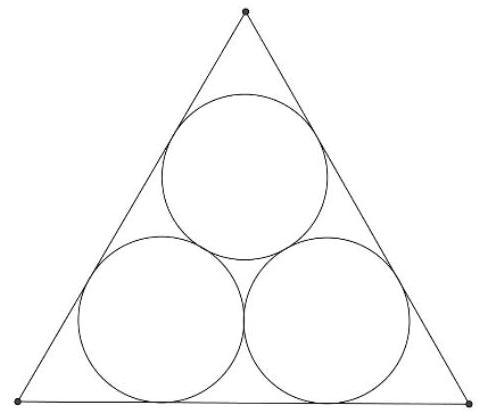
\includegraphics[max width=\textwidth, center]{2024_11_21_4f92067f3905c4fae6dfg-1}
\end{enumerate}

\section*{KLASY TRZECIE I CZWARTE}
\begin{enumerate}
  \item Dane są punkty \(A=(-5,0), B=(-3,-4), C=(3,4), M=(7,1)\). Z punktu \(M\) poprowadzono styczne \(k\) i \(l\) do okręgu opisanego na trójkącie \(A B C\). Oblicz pole trójkąta \(K L M\), gdzie \(K\) i \(L\) są punktami styczności prostych \(k\) i \(l\) z tym okręgiem.
  \item Oblicz sumę \(n\) początkowych wyrazów ciągu \(\left(a_{n}\right)\), w którym \(a_{1}=3, a_{2}=33, a_{3}=333, a_{4}=3333, \ldots\)
  \item W półokrąg o promieniu R wpisano trapez, w którym ramię jest nachylone pod kątem \(\alpha\) do podstawy będącej średnicą okręgu. Oblicz pole trapezu.
\end{enumerate}

\end{document}